\section{调度Kernel和数据移动}
我们需要讨论我们作为并行项目的指挥者的角色。 
并行程序的正确编排是一件美妙的事情——代码全速运行而无需等待数据,
因为我们已经安排了所有数据在正确的时间到达和离开——精心构建的代码可以保持硬件最大程度地忙碌。 这是梦想的组成部分!

快车道上的生活——不仅仅是一条车道!——要求我们认真对待我们作为指挥的工作。 
为了做到这一点,我们可以根据任务图来思考我们的工作。

因此,在本章中,我们将介绍任务图,这是用于正确有效地运行复杂的Kernel序列的机制。 
应用程序中有两件事需要排序:Kernel执行和数据移动。 任务图是我们用来实现正确排序的机制。

首先,我们将快速回顾一下第 3 章中如何使用依赖关系来排序任务。接下来,我们将介绍 SYCL 运行时如何构建图。 
我们将讨论 SYCL 图的基本构建块,即命令组。 然后我们将说明构建常见模式图的不同方法。 
我们还将讨论如何在Graph中表示显式和隐式的数据移动。 最后,我们将讨论将Graph与主机同步的各种方法。


\subsection{什么是图调度?}
在第 3 章中,我们讨论了数据管理和数据使用排序。 该章描述了 SYCL 中图背后的关键抽象:依赖关系。 
Kernel之间的依赖关系基本上基于Kernel访问的数据。 Kernel需要确保它读取了正确的数据,然后才能计算其输出。

我们描述了对于确保正确执行非常重要的三种类型的数据依赖性。 
第一种是写后读 (RAW),当一个任务需要读取另一个任务生成的数据时发生。 这种类型的依赖性描述了两个Kernel之间的数据流。 
当一个任务在另一个任务读取数据后需要更新数据时,就会发生第二种类型的依赖。 
我们将这种类型的依赖关系称为“读后写”(WAR) 依赖关系。 
当两个任务尝试写入相同的数据时,会出现最后一种类型的数据依赖。 这称为写入后写入 (WAW) 依赖性。

数据依赖性是我们用来构建Graph的构建块。 
这组依赖关系是我们表达简单线性Kernel链和包含数百个具有复杂依赖关系的Kernel的大型复杂图所需的全部。 
无论计算需要哪种类型的图,SYCL 图都确保程序将根据所表达的依赖关系正确执行。 
然而,程序员需要确保Graph正确地表达程序中的所有依赖关系。

\subsection{SYCL 中的Graph如何工作}
命令组可以包含三个不同的内容:操作、其依赖项和其他主机代码。 
在这三件事中,始终需要的是行动,因为没有它,指挥组实际上什么也做不了。 
大多数命令组也会表达依赖性,但在某些情况下可能不会。 一个这样的例子是程序中提交的第一个操作。 
它不依赖于任何东西来开始执行; 因此,我们不会指定任何依赖性。 
命令组中可能出现的另一件事是在主机上执行的任意 C++ 代码。 
这是完全合法的,并且对于帮助指定操作或其依赖性很有用,
并且此代码在创建命令组时执行(而不是稍后,当基于已满足的依赖性执行操作时)。

命令组通常表示为传递给提交方法的 C++ lambda 表达式。 
命令组还可以通过队列对象上的快捷方法来表达,该队列对象采用Kernel和基于事件的依赖集。

\subsubsection{命令组行动}
命令组可以执行两种类型的操作:Kernel执行和显式内存操作。 命令组只能执行单个操作。 
正如我们在前面的章节中所看到的,Kernel是通过调用parallel\_for或single\_task方法来定义的,
并表达我们想要在设备上执行的计算。 显式数据移动的操作是第二种类型的操作。 
USM 的示例包括 memcpy、memset 和 fill 操作。 Buffer的示例包括复制、填充和 update\_host。

\subsubsection{命令组如何声明依赖关系}
命令组的另一个主要组成部分是一组依赖关系,在执行该组定义的操作之前必须满足这些依赖关系。 
SYCL 允许以多种方式指定这些依赖性。

如果程序使用有序 SYCL 队列,则队列的有序语义指定连续排队的命令组之间的隐式依赖关系。 
在先前提交的任务完成之前,一项任务无法执行。

基于事件的依赖性是指定命令组执行之前必须完成的操作的另一种方法。 这些基于事件的依赖性可以用两种样式来指定。 
当命令组被指定为传递给队列的提交方法的 lambda 时,使用第一种方法。 
在这种情况下,程序员调用命令组处理程序对象的 dependent\_on 方法,传递事件或事件向量作为参数。 
当从队列对象上定义的快捷方法创建命令组时,使用另一种方法。 
当程序员直接在队列上调用parallel\_for或single\_task时,事件或事件向量可以作为额外参数传递。

指定依赖关系的最后一种方法是通过创建访问器对象。 
访问器指定如何使用它们来读取或写入Buffer对象中的数据,让运行时使用此信息来确定不同Kernel之间存在的数据依赖性。

正如我们在本章开头所回顾的,数据依赖的示例包括一个Kernel读取另一个Kernel生成的数据、两个Kernel写入相同的数据,
或者一个Kernel在另一个Kernel读取数据后修改数据。

\subsubsection{例子}
现在我们将通过几个例子来说明我们刚刚学到的一切。 我们将展示如何以多种方式表达两种不同的依赖模式。 
我们将说明的两种模式是线性依赖链(其中一个任务在另一个任务之后执行)
和“Y”模式(其中两个独立任务必须在连续任务之前执行)。

\begin{figure}[H]
	\centering
	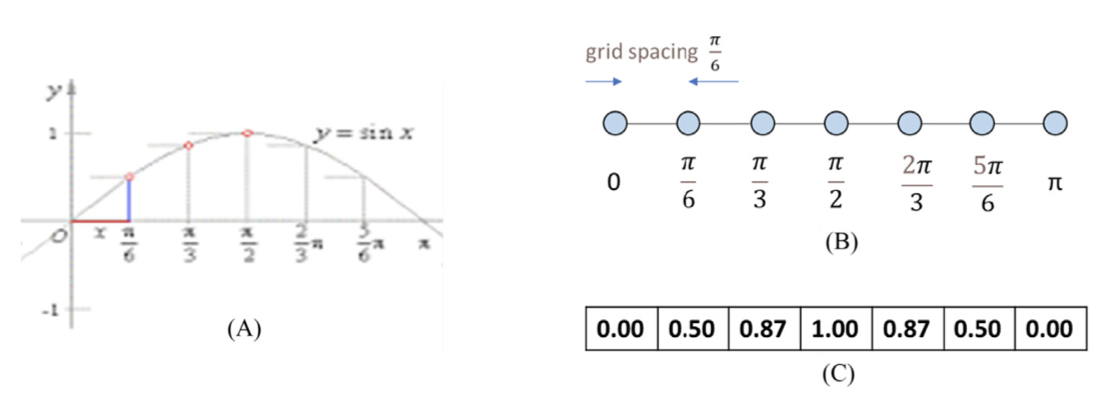
\includegraphics[width=0.9\textwidth]{figs/F8.1.png}
	\caption{\textit{线性依赖链图 }}
\end{figure}

\begin{figure}[H]
	\centering
	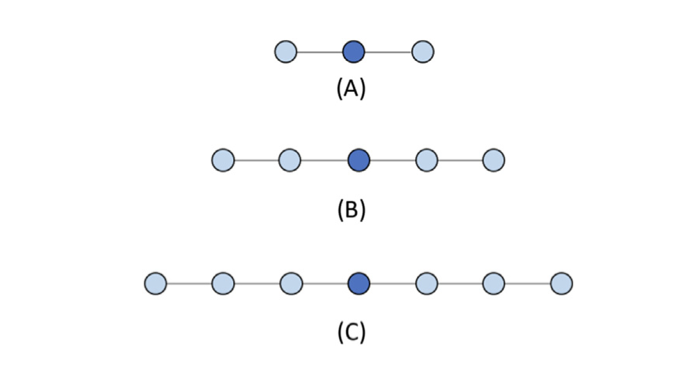
\includegraphics[width=0.9\textwidth]{figs/F8.2.png}
	\caption{\textit{“Y”模式依赖关系图 }}
\end{figure}

这些依赖模式的Graph如图 8-1 和 8-2 所示。 图 8-1 描述了一个线性依赖链。 
第一个节点表示数据的初始化,而第二个节点表示将数据累积为单个结果的归约操作。 
图 8-2 描绘了一个“Y”模式,其中我们独立地初始化两个不同的数据。 数据初始化后,加法Kernel会将两个向量相加。 
最后,图中的最后一个节点将结果累积为单个值。

对于每种模式,我们将展示三种不同的实现。 第一个实现将使用有序队列。 第二个将使用基于事件的依赖关系。 
最后一个实现将使用Buffer和访问器来表达命令组之间的数据依赖性。

\begin{figure}[H]
	\centering
	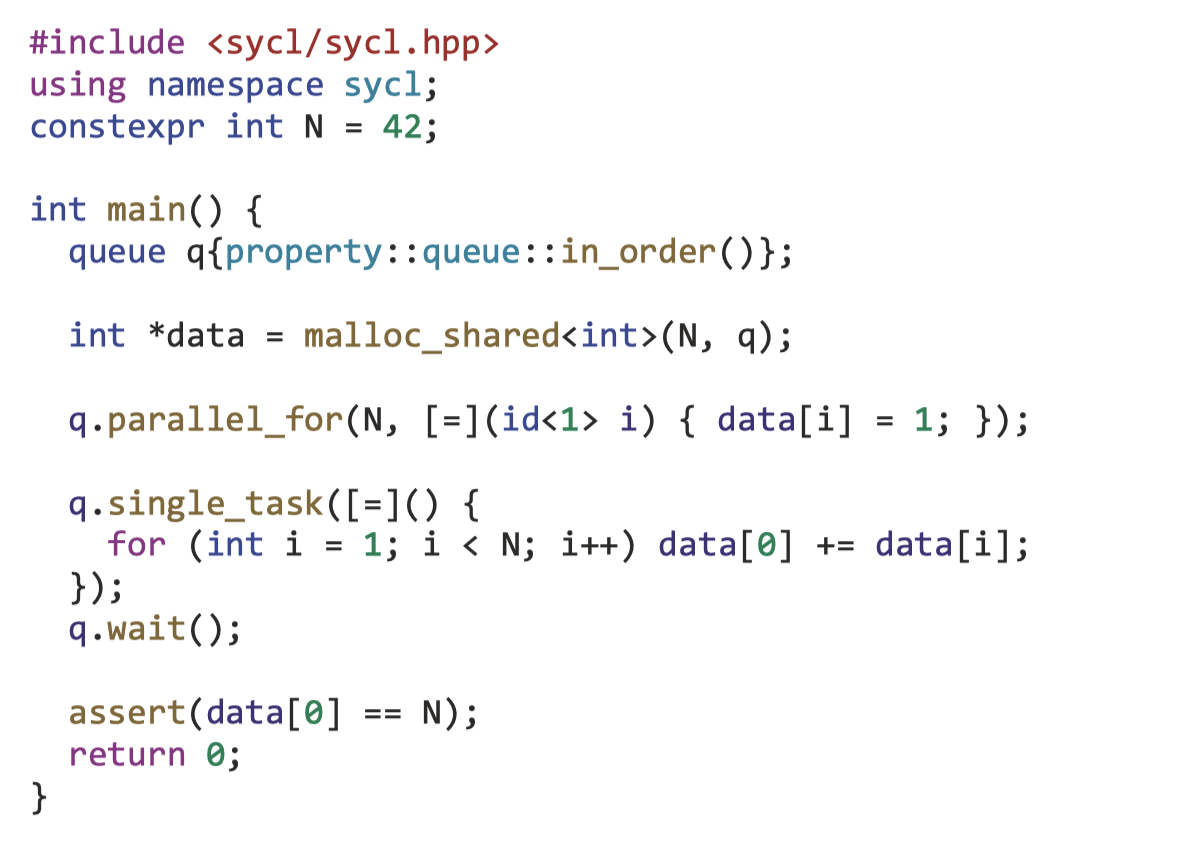
\includegraphics[width=0.9\textwidth]{figs/F8.3.png}
	\caption{\textit{具有顺序队列的线性依赖链 }}
\end{figure}

图 8-3 显示了如何使用有序队列来表达线性依赖链。 这个例子非常简单,因为中序队列的语义已经保证了命令组之间执行的顺序。 
我们提交的第一个Kernel将数组的元素初始化为 1。然后下一个Kernel获取这些元素并将它们相加到第一个元素中。 
由于我们的队列是有序的,因此我们不需要做任何其他事情来表示第二个Kernel在第一个Kernel完成之前不应执行。 
最后,我们等待队列完成执行所有任务,并检查是否获得了预期结果。

\begin{figure}[H]
	\centering
	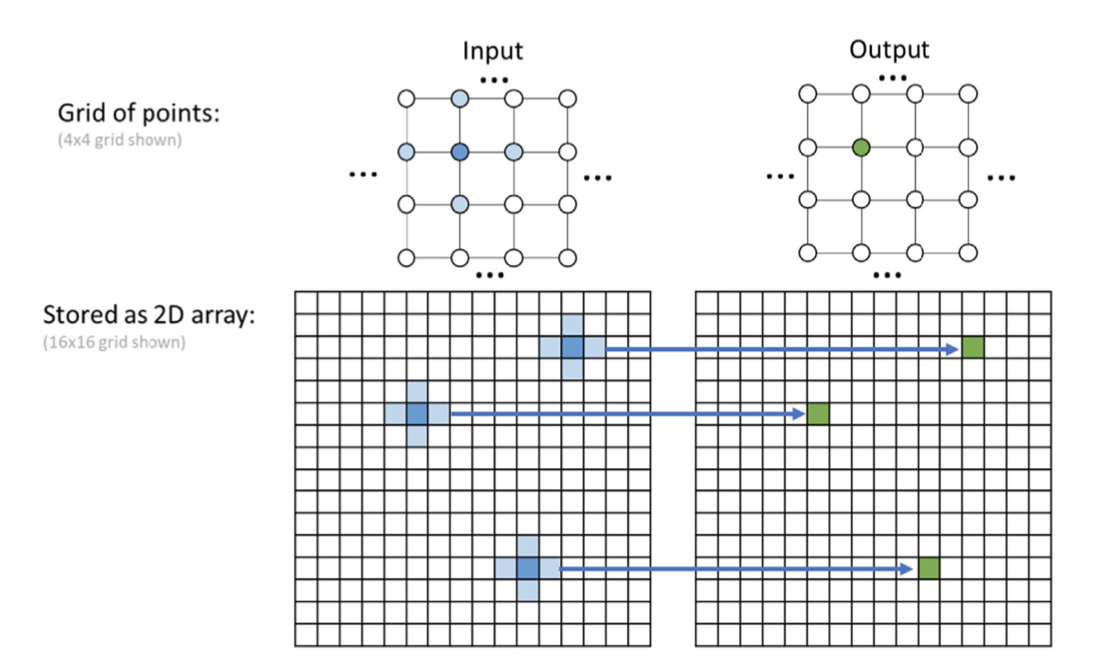
\includegraphics[width=0.9\textwidth]{figs/F8.4.png}
	\caption{\textit{事件的线性依赖链 }}
\end{figure}

图 8-4 显示了使用无序队列和基于事件的依赖关系的同一示例。 在这里,我们捕获第一次调用 parallel\_for 返回的事件。 
然后,第二个Kernel能够通过将其作为参数传递给depends\_on来指定对该事件及其代表的Kernel执行的依赖。 
我们将在图 8-6 中看到如何使用定义Kernel的快捷方法之一来缩短第二个Kernel的表达式。

\begin{figure}[H]
	\centering
	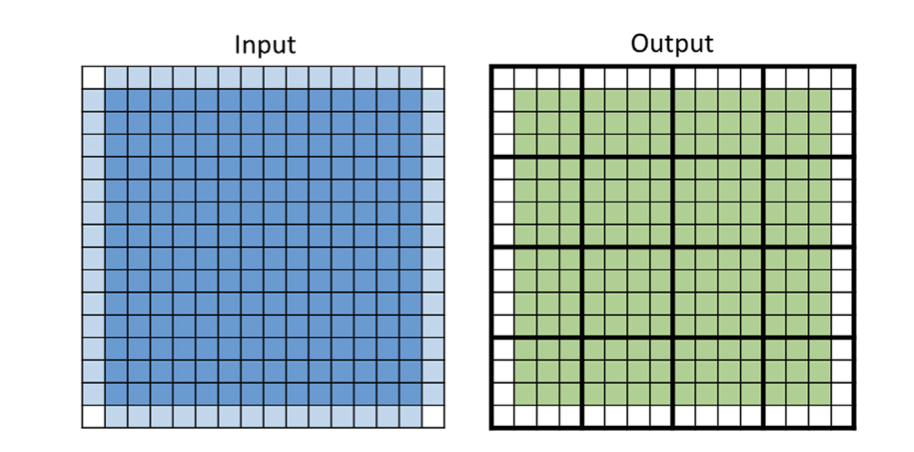
\includegraphics[width=0.9\textwidth]{figs/F8.5.png}
	\caption{\textit{具有Buffer和访问器的线性依赖链 }}
\end{figure}

图 8-5 使用Buffer和访问器而不是 USM 指针重写了我们的线性依赖链示例。 
在这里,我们再次使用无序队列,但使用通过访问器指定的数据依赖性而不是基于事件的依赖性来排序命令组的执行。 
第二个Kernel读取第一个Kernel生成的数据,运行时可以看到这一点,因为我们基于相同的底层Buffer对象声明访问器。 
与前面的示例不同,我们不会等待队列完成执行所有任务。 
相反,我们构建一个主机访问器,定义第二个Kernel的输出与我们在主机上计算出正确答案的断言之间的数据依赖关系。 
请注意,虽然主机访问器为我们提供了主机上数据的最新视图,但如果在创建Buffer时指定了任何内容,
它并不能保证原始主机内存已更新。 
我们无法安全地访问原始主机内存,除非Buffer首先被破坏,或者除非我们使用更高级的机制,如第 7 章中描述的互斥机制。

\begin{figure}[H]
	\centering
	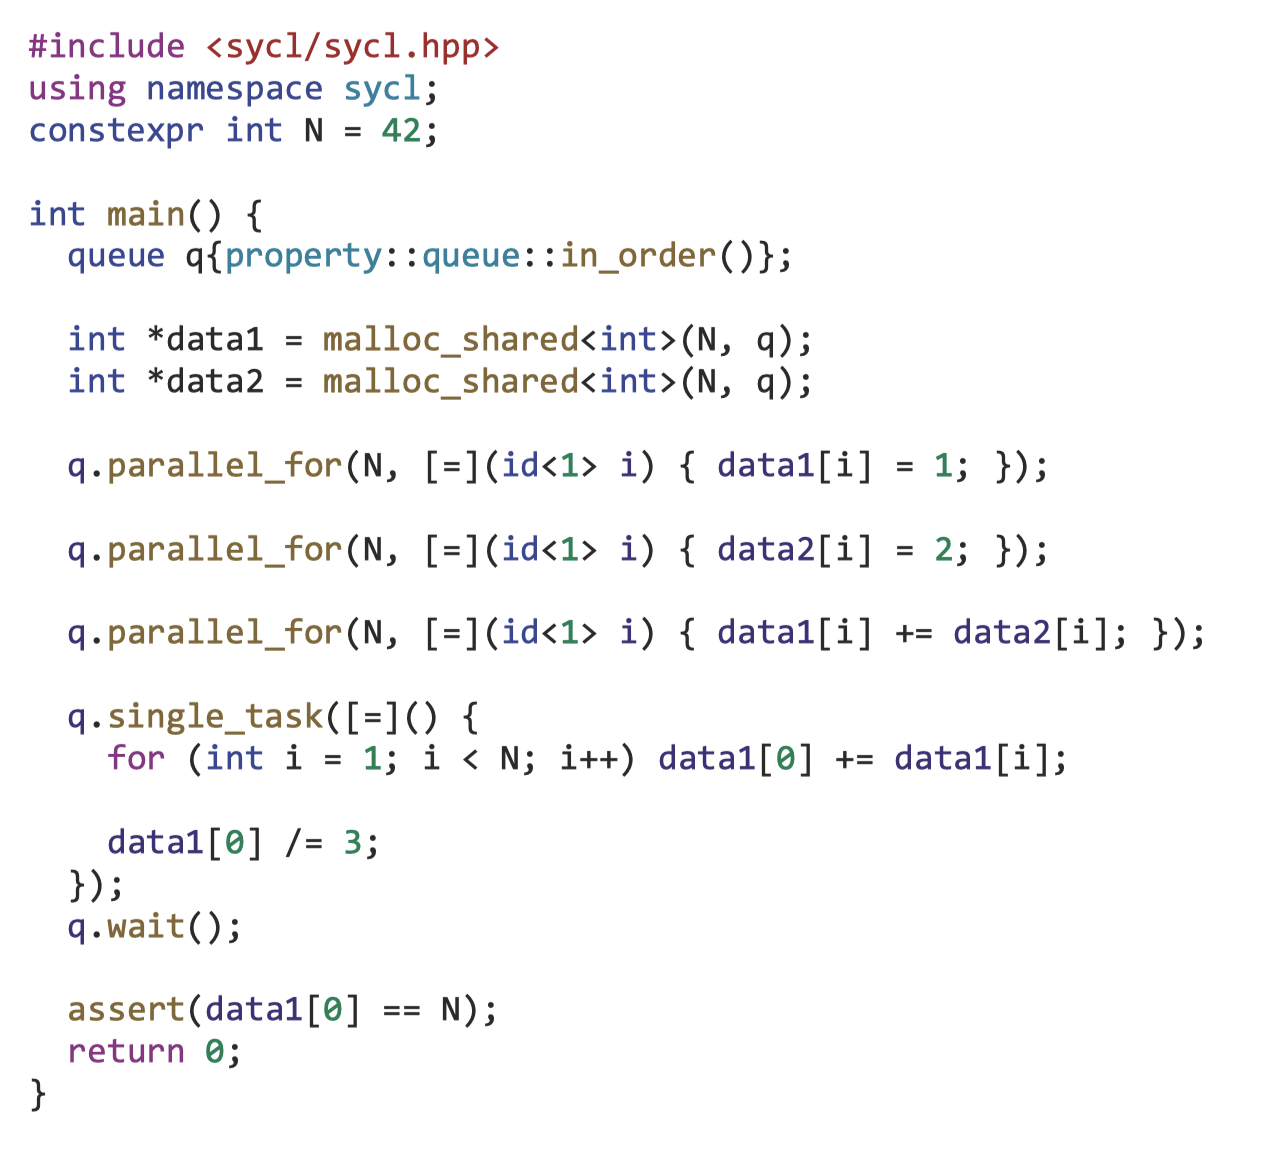
\includegraphics[width=0.9\textwidth]{figs/F8.6.png}
	\caption{\textit{具有顺序队列的“Y”模式 }}
\end{figure}

图 8-6 显示了如何使用有序队列表达“Y”模式。 在此示例中,我们声明两个数组:data1 和 data2。 
然后,我们定义两个Kernel,每个Kernel将初始化其中一个数组。 
这些Kernel彼此不依赖,但由于队列是有序的,因此Kernel必须一个接一个地执行。 
请注意,在此示例中交换这两个Kernel的顺序是完全合法的。 
第二个Kernel执行后,第三个Kernel将第二个数组的元素添加到第一个数组的元素中。 
最终Kernel对第一个数组的元素进行求和,以计算与我们在线性相关链示例中所做的相同结果。 
这个求和Kernel依赖于之前的Kernel,但是这个线性链也被有序队列捕获。 
最后,我们等待所有Kernel完成并验证我们是否成功计算了幻数。

\begin{figure}[H]
	\centering
	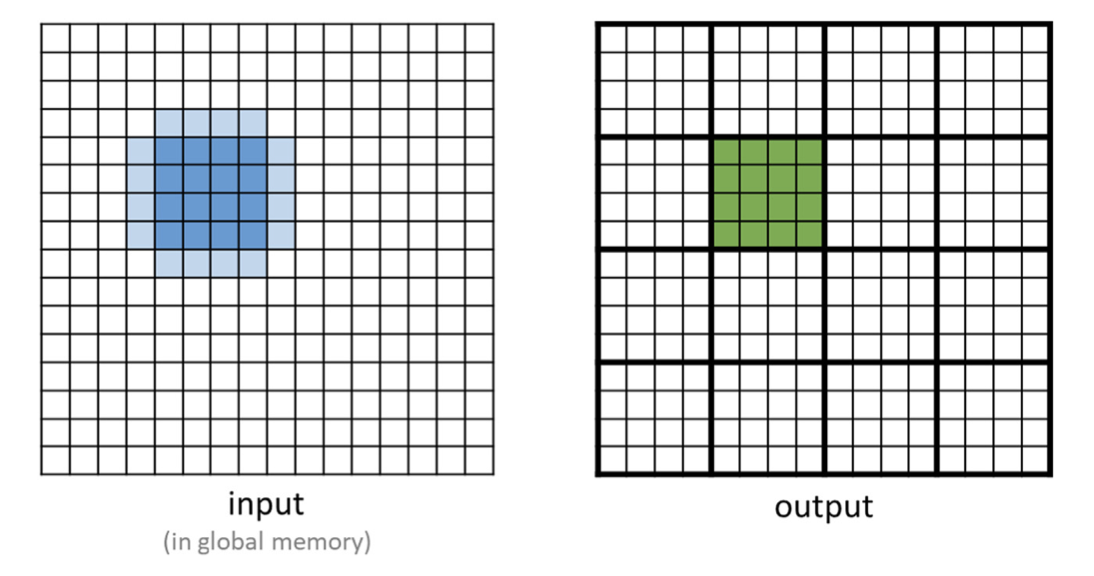
\includegraphics[width=0.9\textwidth]{figs/F8.7.png}
	\caption{\textit{带有事件的“Y”模式 }}
\end{figure}

图 8-7 显示了我们的“Y”模式示例,其中使用无序队列而不是有序队列。 
由于队列的顺序导致依赖关系不再是隐式的,因此我们必须使用事件显式指定命令组之间的依赖关系。 
如图 8-6 所示,我们首先定义两个没有初始依赖性的独立Kernel。 我们用两个事件 e1 和 e2 来表示这些Kernel。 
当我们定义第三个Kernel时,我们必须指定它依赖于前两个Kernel。 
我们通过说它取决于事件 e1 和 e2 在执行之前完成来做到这一点。 
然而,在这个例子中,我们使用快捷形式来指定这些依赖关系,而不是处理程序的depends\_on方法。 
在这里,我们将事件作为额外参数传递给parallel\_for。 
由于我们想要一次传递多个事件,因此我们使用接受事件 std::vector 的形式,
但幸运的是,现代 C++ 通过自动将表达式 {e1, e2} 转换为适当的向量,为我们简化了这一过程。

\begin{figure}[H]
	\centering
	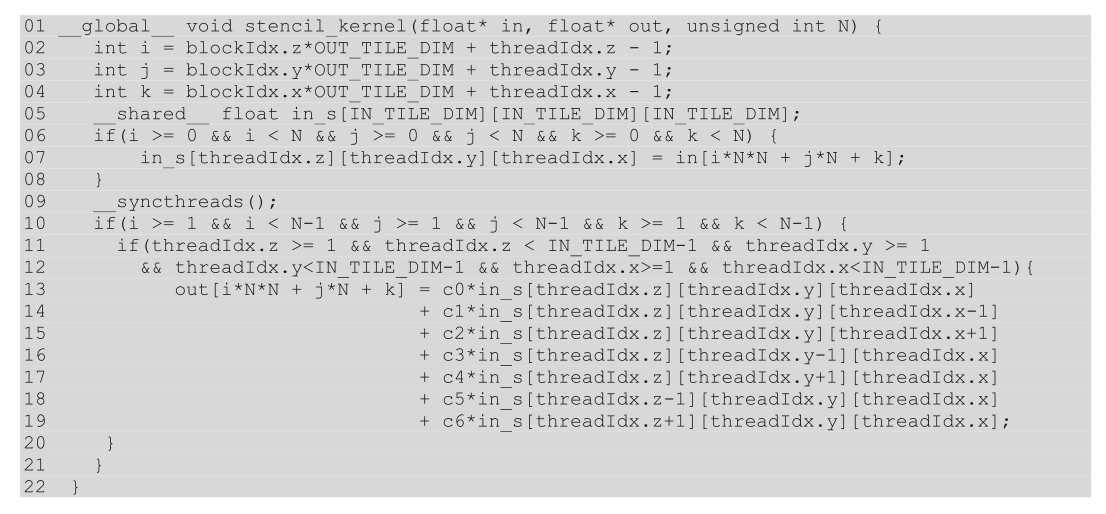
\includegraphics[width=0.9\textwidth]{figs/F8.8.png}
	\caption{\textit{带访问器的“Y”型模式 }}
\end{figure}

在我们的最后一个示例中,如图 8-8 所示,我们再次用Buffer和访问器替换 USM 指针和事件。 
此示例将两个数组 data1 和 data2 表示为Buffer对象。 
我们的Kernel不再使用快捷方法来定义Kernel,因为我们必须将访问器与命令组处理程序关联起来。 
再一次,第三个Kernel必须捕获对前两个Kernel的依赖。 这里这是通过声明Buffer的访问器来完成的。 
由于我们之前已经声明了这些Buffer的访问器,因此运行时能够正确排序这些Kernel的执行。 
此外,当我们声明访问器 b 时,我们还向运行时提供额外的信息。 
我们添加访问标记 read\_only 让运行时知道我们只会读取这些数据,不会生成新值。 
正如我们在线性依赖链的Buffer和访问器示例中看到的那样,
我们的最终Kernel通过更新第三个Kernel中生成的值来对自身进行排序。 
我们通过声明一个主机访问器来检索计算的最终值,
该主机访问器将等待最终Kernel完成执行,然后将数据移回主机,在主机上我们可以读取数据并断言我们计算了正确的结果。

\subsubsection{命令组的各个部分何时执行?}
由于任务图是异步的,因此有必要了解命令组的确切执行时间。 
到目前为止,应该清楚的是,一旦满足了Kernel的依赖性,就可以执行Kernel,但是命令组的主机部分会发生什么情况呢?

当命令组提交到队列时,它会立即在主机上执行(在提交调用返回之前)。 
命令组的该主机部分仅执行一次。 命令组中定义的任何Kernel或显式数据操作都会排队在设备上执行。

\subsection{数据移动}
数据移动是 SYCL 中Graph的另一个非常重要的方面,这对于理解应用程序性能至关重要。 
但是,如果数据移动在程序中隐式发生(使用Buffer和访问器或使用 USM 共享分配),则通常会意外地忽略这一点。 
接下来,我们将研究数据移动影响 SYCL 中Graph执行的不同方式。

\subsubsection{显式数据移动}
显式数据移动的优点是它显式地出现在Graph中,使程序员可以清楚地了解Graph执行过程中发生的情况。 
我们将显式数据操作分为 USM 和Buffer的操作。

正如我们在第 6 章中了解到的,当我们需要在设备分配和主机之间复制数据时,USM 中会发生显式数据移动。 
这是通过队列和处理程序类中的 memcpy 方法完成的。 
提交操作或命令组会返回一个事件,该事件可用于与其他命令组一起订购副本。

通过调用命令组处理程序对象的 copy 或 update\_host 方法,可以通过Buffer进行显式数据移动。

复制方法可用于在主机内存和设备上的访问器对象之间手动交换数据。 这样做可以出于多种原因。 
一个简单的例子是对长时间运行的计算序列设置检查点。 使用复制方法,数据可以以单向方式从设备写入任意主机存储器。 
如果使用Buffer完成此操作,则大多数情况(即Buffer不是使用 use\_host\_ptr 创建的)将需要首先将数据复制到主机,
然后从Buffer的内存复制到所需的主机内存。

update\_host 方法是一种非常特殊的复制形式。 
如果围绕主机指针创建Buffer,则此方法会将访问器表示的数据复制回原始主机内存。 
如果程序手动将主机数据与使用特殊 use\_mutex 属性创建的Buffer同步,这会很有用。 
然而,这种用例在大多数程序中不太可能出现。

\subsubsection{隐式数据移动}
隐式数据移动可能会对 SYCL 中的命令组和任务图产生隐藏的后果。 
通过隐式数据移动,数据可以通过 SYCL 运行时或通过硬件和软件的某种组合在主机和设备之间复制。 
无论哪种情况,复制都会在没有用户明确输入的情况下发生。 让我们再次分别看看 USM 和缓冲器的情况。

使用 USM,主机和共享分配会发生隐式数据移动。 
正如我们在第 6 章中了解到的,主机分配实际上并不移动数据,而是远程访问数据,并且共享分配可能会在主机和设备之间迁移。 
由于此迁移是自动发生的,因此 USM 隐式数据移动和命令组实际上无需考虑。 
然而,共享分配有一些细微差别值得记住。

预取操作的工作方式与 memcpy 类似,以便让运行时在Kernel尝试使用共享分配之前开始迁移它们。 
然而,与必须复制数据以确保正确结果的 memcpy 不同,预取通常被视为运行时的提示以提高性能,
并且预取不会使内存中的指针值无效(就像复制到新地址范围时那样) )。 
如果在Kernel开始执行之前预取尚未完成,程序仍将正确执行,
并且许多代码可能选择使图中的命令组不依赖于预取操作,因为它们不是功能要求。

Buffer也有一些细微差别。 使用Buffer时,命令组必须为Buffer构造访问器,以指定如何使用数据。 
这些数据依赖性表达了不同命令组之间的顺序,并允许我们构建任务图。 
然而,带有Buffer的命令组有时还具有另一个目的:它们指定数据移动的要求。

访问器指定Kernel将读取或写入Buffer。 由此推论,数据也必须在设备上可用,如果不可用,
则运行时必须在Kernel开始执行之前将其移动到那里。 
因此,SYCL 运行时必须跟踪Buffer当前版本所在的位置,以便可以安排数据移动操作。 
访问器创建有效地在图中创建了一个额外的隐藏节点。 如果需要数据移动,运行时必须首先执行它。 
只有这样,提交的Kernel才能执行。

让我们再看一下图8-8。 在此示例中,我们的前两个Kernel将需要将Buffer data1 和 data2 复制到设备; 
运行时隐式创建额外的Graph节点来执行数据移动。 
当第三个Kernel的命令组被提交时,这些Buffer很可能仍然在设备上,因此运行时不需要执行任何额外的数据移动。 
第四个Kernel的数据也可能不需要任何额外的数据移动,
但主机访问器的创建需要运行时在访问器可供使用之前安排将Buffer数据1移动回主机。

\subsection{与主机同步}
我们要讨论的最后一个主题是如何与主机同步图执行。 
我们已经在整章中谈到了这一点,但现在我们将研究程序执行此操作的所有不同方式。

主机同步的第一种方法是我们在前面的许多示例中使用的方法:等待队列。 
队列对象有两个方法:wait 和 wait\_and\_throw,它们会阻止主机执行,直到提交到队列的每个命令组完成为止。 
这是一个非常简单的方法,可以处理许多常见情况。 然而,值得指出的是,这种方法的粒度非常粗。 
如果需要更细粒度的同步(例如,可能提高性能),我们将讨论的其他方法之一可能更适合应用程序的需求。

主机同步的下一个方法是同步事件。 这为队列同步提供了更大的灵活性,因为它允许应用程序仅在特定操作或命令组上同步。 
这是通过调用事件的 wait 方法或调用事件类的静态方法 wait 来完成的,该事件类可以接受事件向量。

我们已经看到图 8-5 和 8-8 中使用的下一个方法:主机访问器。 主机访问器执行两个功能。 
首先,顾名思义,它们使数据可在主机上访问。 其次,它们通过定义当前访问的图和主机之间的新依赖关系来同步设备和主机。 
这可确保复制回主机的数据具有Graph正在执行的计算的正确值。 
然而,我们再次注意到,如果Buffer是从现有主机内存构造的,则不能保证该原始内存包含更新的值。

请注意,主机访问器是阻塞的。 在数据可用之前,主机上的执行可能不会超过主机访问器的创建。 
同样,当主机访问器存在并保持其数据可用时,Buffer不能在设备上使用。 
一种常见的模式是在附加 C++ 作用域内创建主机访问器,以便在不再需要主机访问器时释放数据。 
这是下一个主机同步方法的示例。

SYCL 中的某些对象在被销毁时具有特殊行为,并调用其析构函数。 
我们刚刚了解了主机访问器如何使数据保留在主机上直到它们被销毁。 
当Buffer和图像被破坏或离开范围时,它们也有特殊的行为。 
当Buffer被销毁时,它会等待所有使用该Buffer的命令组完成执行。 
一旦Buffer不再被任何Kernel或内存操作使用,运行时可能必须将数据复制回主机。 
如果使用主机指针初始化Buffer或将主机指针传递给方法 set\_final\_data,则会发生此复制。 
然后,运行时将复制回该Buffer的数据并在对象被销毁之前更新主机指针。

与主机同步的最后一个选项涉及第 7 章中首先描述的一个不常见的功能。
回想一下,Buffer对象的构造函数可以选择采用属性列表。 
创建Buffer时可以传递的有效属性之一是 use\_mutex。 
当以这种方式创建Buffer时,它增加了Buffer拥有的内存可以与主机应用程序共享的要求。 
对该内存的访问由用于初始化Buffer的互斥体控制。 
当可以安全地访问与Buffer共享的内存时,主机能够获得互斥体上的锁。 
如果无法获得锁,用户可能需要排队内存移动操作来与主机同步数据。 
这种用途非常特殊,在大多数 DPC++ 应用程序中不太可能找到。

\subsection{总结}
在本章中,我们了解了图以及它们如何在 SYCL 中构建、调度和执行。 
我们详细介绍了指挥组的含义以及它们的功能。 
我们讨论了命令组中可以包含的三件事:依赖性、操作和其他主机代码。 
我们回顾了如何使用事件以及通过访问器描述的数据依赖性来指定任务之间的依赖性。 
我们了解到命令组中的单个操作可能是Kernel或显式内存操作,然后我们查看了几个示例,
这些示例展示了构建常见执行图模式的不同方法。 
接下来,我们回顾了数据移动如何成为 SYCL 图的重要组成部分,并了解了它如何显式或隐式地出现在图中。 
最后,我们研究了将图的执行与主机同步的所有方法。

了解程序流程可以使我们了解在调试运行时失败时可以打印的调试信息类型。 
第 13 章“调试运行时故障”部分有一个表格,考虑到我们在本书中这一点所获得的知识,该表格会更有意义。 
然而,本书并不试图详细讨论这些高级编译器转储。

希望这让您感觉自己像一位Graph专家,可以构建各种复杂程度的Graph,
从线性链到具有数百个节点以及复杂数据和任务依赖性的巨大Graph! 
在下一章中,我们将开始深入研究有助于提高特定设备上应用程序性能的底层细节。